\clearpage
\usetikzlibrary{automata, arrows.meta, positioning}
%//==============================--@--==============================//%
%\vspace{-1em}
\subsection{P4 | Diagrama de transição modificado.}
\label{subsec:P4}

De modo a emular a permanência no estado prisão durante uma jogada, acrescenta-se um estado \textit{dummy}, denomidado por $x_P$, para o qual se transita, (possivelmente) dos estados $5$ ou $6$. Nestes moldes, uma jogada é desperdiçada entre a transição obrigatória do estado $x_P$ para o estado $3$ (transição esta \underline{independente do resultado do lançamento da moeda}).

\begin{figure}[H]
    \centering
    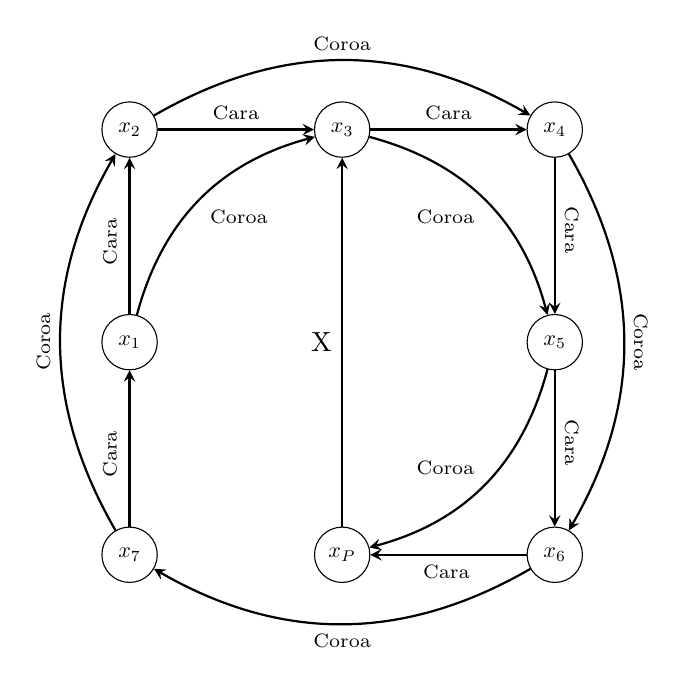
\begin{tikzpicture}[node distance = 2.7cm, on grid, auto, transform shape]
    
        \node (1) [state, scale=0.8, transform shape] {$x_1$};
        \node (2) [state, above = of 1, scale=0.8, transform shape] {$x_2$};
        \node (3) [state, right = of 2, scale=0.8, transform shape] {$x_3$};
        \node (4) [state, right = of 3, scale=0.8, transform shape] {$x_4$};
        \node (5) [state, below = of 4, scale=0.8, transform shape] {$x_5$};
        \node (6) [state, below = of 5, scale=0.8, transform shape] {$x_6$};
        \node (7) [state, below = of 1, scale=0.8, transform shape] {$x_7$};
        \node (8) [state, left = of 6, scale=0.8, transform shape] {$x_P$};
    
        \path [-stealth, thick]
            (1) edge node [left, rotate=90, xshift=0.35cm, yshift = 0.25cm, transform shape] {\scriptsize Cara} (2)
            (2) edge node [above, transform shape] {\scriptsize Cara} (3)
            (3) edge node [above, transform shape] {\scriptsize Cara} (4)
            (4) edge node [above right, rotate=-90, xshift=-0.5cm, transform shape] {\scriptsize Cara} (5)
            (5) edge node [above right, rotate=-90, xshift=-0.5cm, transform shape] {\scriptsize Cara} (6)
            (6) edge [bend left = 30, transform shape] node [below, transform shape] {\scriptsize Coroa} (7)
            (7) edge node [left, rotate=90,xshift=0.35cm, yshift = 0.25cm, transform shape] {\scriptsize Cara} (1)
            (1) edge [bend left = 30, transform shape] node [below right] {\scriptsize Coroa} (3)
            (2) edge [bend left = 30, transform shape] node [above] {\scriptsize Coroa} (4)
            (3) edge [bend left = 30, transform shape] node [below left] {\scriptsize Coroa} (5)
            (4) edge [bend left = 30, transform shape] node [above right, rotate=-90, xshift = -0.5cm] {\scriptsize Coroa} (6)
            (7) edge [bend left = 30, transform shape] node [above left, rotate=90, xshift=0.5cm] {\scriptsize Coroa} (2)
            (5) edge [bend left = 30, transform shape] node [above left] {\scriptsize Coroa} (8)
            (6) edge node [below left, xshift=0.4cm] {\scriptsize Cara} (8)
            (8) edge node [left] {X} (3);
            
    \end{tikzpicture}
    \caption{Diagrama de transição de estados modificado com a introdução de um \textit{dummy state}, de modo a descartar uma possível jogada, na eventualidade do jogador ser enviado para a prisão.}
    \label{fig:P4}
\end{figure}

Seguindo o mesmo raciocínio, é trivialmente generalizado o esquema para um número arbitrário de jogadas em que se pretende que o jogador permaneça no estado prisão. Esta façanha é concretizável introduzindo os \textit{dummy states} desejáveis entre o estado $x_p$ e o estado $3$, de forma a gastar jogadas com estas transições impostas (sempre \underline{independentes do lançamento da moeda}). 

\iffalse
\noindent Complementa-se o diagrama com a matriz de transição $\pmb{P}$ respetiva:
$$
\pmb{P}=
    \begin{bmatrix}
        0 & 0.5 & 0.5 & 0 & 0 & 0 & 0 & 0\\
        0 & 0 & 0.5 & 0.5 & 0 & 0 & 0 & 0\\
        0 & 0 & 0 & 0.5 & 0.5 & 0 & 0 & 0\\
        0 & 0 & 0 & 0 & 0.5 & 0.5 & 0 & 0\\
        0 & 0 & 0 & 0 & 0 & 0.5 & 0 & 0.5\\
        0 & 0 & 0 & 0 & 0 & 0 & 0.5 & 0.5\\
        0.5 & 0.5 & 0 & 0 & 0 & 0 & 0 & 0\\
        0 & 0 & 1 & 0 & 0 & 0 & 0 & 0
    \end{bmatrix}
$$
\fi
%//==============================--@--==============================//%